\documentclass{standalone}
\usepackage[dvipsnames]{xcolor} % braucht diese Reihenfolge ffs
\usepackage{tikz}
\usetikzlibrary{graphs, quotes}

\begin{document}
    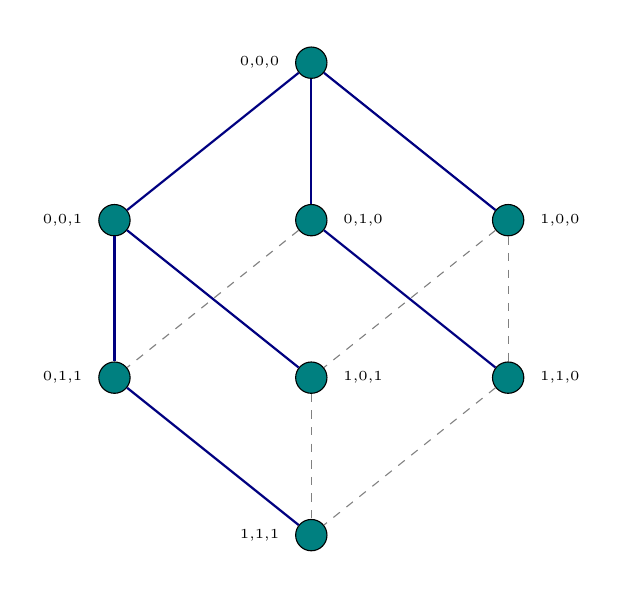
\begin{tikzpicture}[
    node distance = 4cm and 4cm,
    V/.style = {circle, draw, fill=teal, inner sep = 4pt, font=\tiny},
    every edge quotes/.style = {auto, font=\footnotesize}
    ]
    \begin{scope}[nodes=V]
        \node[label=left:{0,0,0}] (000) at (0,0) {};
        \node[label=left:{0,0,1}] (001) at (-2.5,-2) {};
        \node[label=right:{0,1,0}] (010) at (0,-2) {};
        \node[label=right:{1,0,0}] (100) at (2.5,-2) {};
        \node[label=left:{0,1,1}] (011) at (-2.5,-4) {};
        \node[label=right:{1,0,1}] (101) at (0,-4) {};
        \node[label=right:{1,1,0}] (110) at (2.5,-4) {};
        \node[label=left:{1,1,1}] (111) at (0,-6) {};
    \end{scope}
    \begin{scope}[every edge/.style=draw, thick, NavyBlue]
        \draw (000) -- (001);
        \draw (000) -- (010);
        \draw (000) -- (100);
        \draw (001) -- (011);
        \draw (001) -- (101);
        \draw (010) -- (110);
        \draw (011) -- (111);
    \end{scope}
    \begin{scope}[every edge/.style=draw, dashed, thin, gray]
        \draw (010) -- (011);
        \draw (100) -- (110);
        \draw (100) -- (101);
        \draw (110) -- (111);
        \draw (101) -- (111);
    \end{scope}
\end{tikzpicture}
\end{document}